% XeLaTeX

\documentclass{article}
\usepackage{ctex}
\usepackage{xypic}
\usepackage{amsfonts,amssymb}
\usepackage{multirow}
\usepackage{geometry}
\usepackage{graphicx}
\usepackage{listings}
\usepackage{lipsum}
\usepackage{courier}
\usepackage{fancyvrb}
\usepackage{etoolbox}


\linespread{1.2}
\geometry{left=3cm,right=2.5cm,top=2.5cm,bottom=2.5cm}

\makeatletter
\patchcmd{\FV@SetupFont}
  {\FV@BaseLineStretch}
  {\fontencoding{T1}\FV@BaseLineStretch}
  {}{}
\makeatother

\lstset{basicstyle=\small\fontencoding{T1}\ttfamily,breaklines=true}
\lstset{numbers=left,frame=shadowbox,tabsize=4}
%\lstset{extendedchars=false}
\begin{document}

\title{数据库系统实验5 \ 实验报告}
\author {数据科学与计算机学院 \ 计算机科学与技术 2016 级 \\ 王凯祺 \ 16337233}
\maketitle

\section{实验5 数据库设计实验}

设计一个图书馆的数据库。其中,一个读者能借多本书,一个管理员可以管理多个读者,可以管理多本书。利用 PowerDesigner 或 ERwin 等数据库设计工具设计该数据库。

\subsection{数据库概念结构设计}

识别出读者 Reader 、管理员 Admin 、书本 Book 共计 3 个实体。每个实体的属性、码如下:

\begin{itemize}
\item 读者 Reader:读者学号(ID)、读者姓名(name)、读者性别(gender)、联系电话(phone)、所在系(department)、累计违章次数(penalty)、累计借书数(borrowed\_book)、备注(remark)。其中主键为读者学号(ID)。
\item 管理员 Admin:管理员工作号(ID)、姓名(name)、性别(gender)、电话(phone)、家庭住址(address)、备注(remark)。其中主键为管理员工作号(ID)。
\item 书本 Book:索书号(ID)、ISBN(ISBN)、分类(class)、书名(title)、作者(author)、出版社(press)、出版日期(publish\_date)、简介(intro)、备注(remark)。其中主键为索书号(ID)。
\end{itemize}

在书本 Book 表中,由于在图书馆中可能会存在两本一模一样的书(ISBN也相同),故有函数依赖 $ID \rightarrow ISBN, remark$ , $ISBN \rightarrow class, title, author, press, publish\_date, intro$ ,不满足 BC 范式。因此我将该表拆为下列二表:

\begin{itemize}
\item 书本 Book:索书号(ID)、ISBN(ISBN)、备注(remark)。其中主键为索书号(ID)。
\item 书籍信息 BookInfo:ISBN(ISBN)、分类(class)、书名(title)、作者(author)、出版社(press)、出版日期(publish\_date)、简介(intro)。其中主键为 ISBN(ISBN)。
\end{itemize}

我们分析各实体之间的关系:借阅关系(书本、读者和操作管理员的多对多对多的关系)。管理员与书本的关系、管理员与读者的关系在图书馆数据库的实际应用中没有体现,不予构建。

实体-联系图(E-R图)如下:

\newpage

\begin{figure}[!h]
\centering
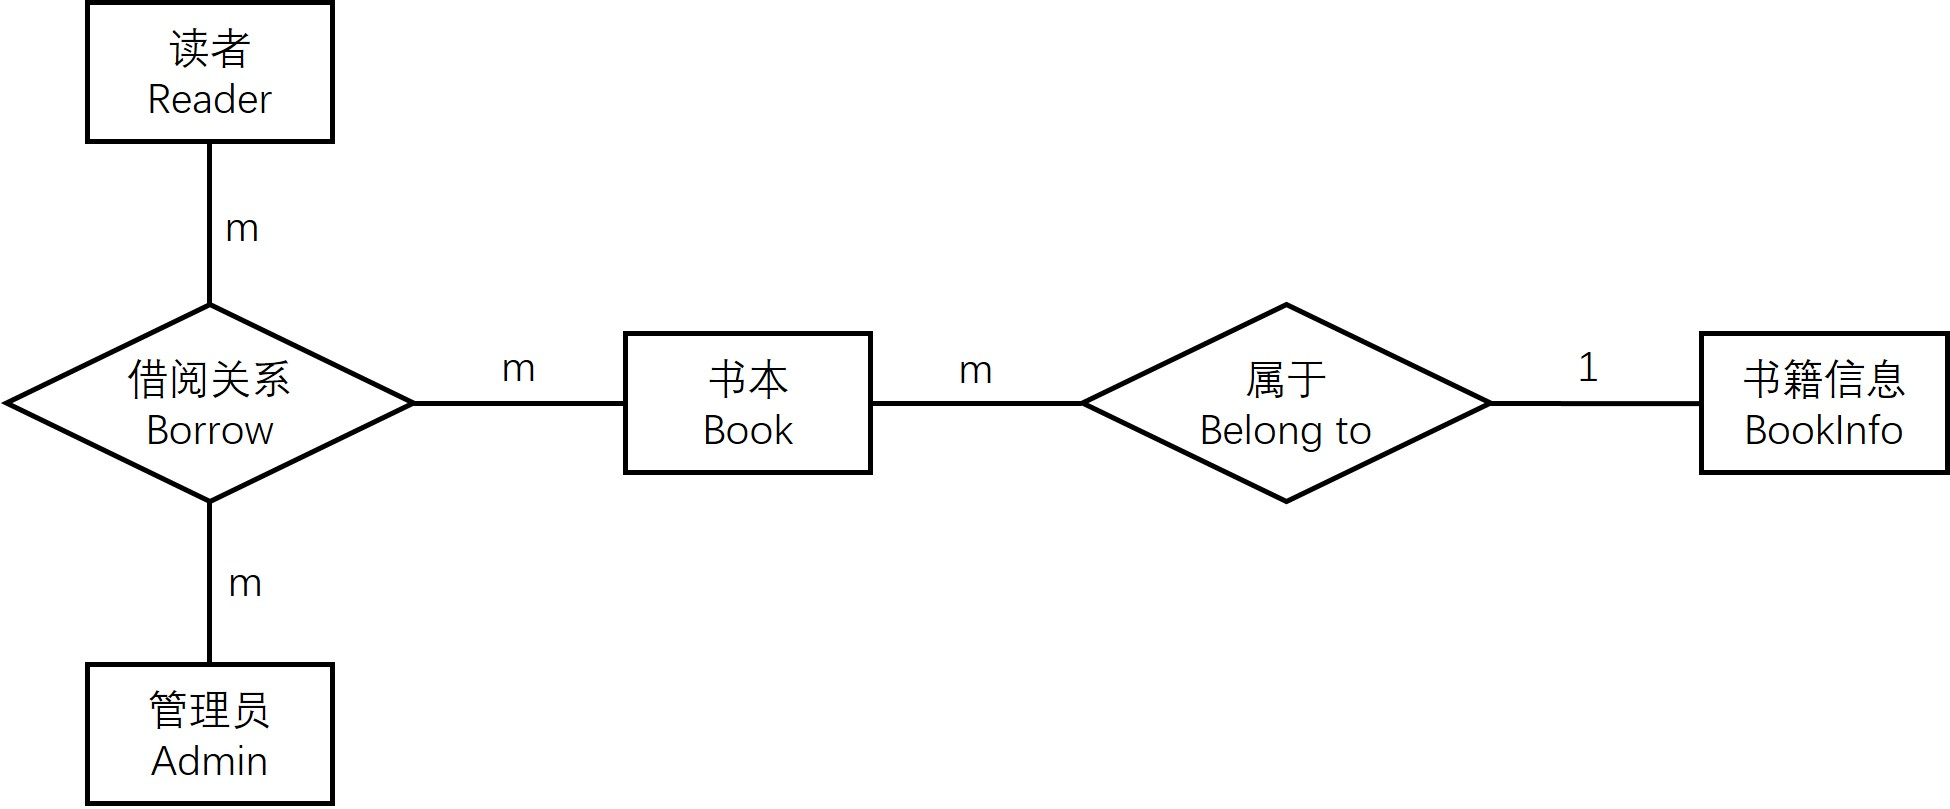
\includegraphics[scale=0.5]{db_imgs/er.jpg}
\end{figure}

\subsection{数据库逻辑结构设计}

按照数据库设计原理中概念结构转化成逻辑结构的规则,每个实体转换成一个关系,多对多的关系也转换成一个关系。因此,根据上述 E-R 图设计数据库逻辑结构。

我使用 Datablau 软件来构建逻辑结构图。逻辑结构图如下:

\begin{figure}[!h]
\centering
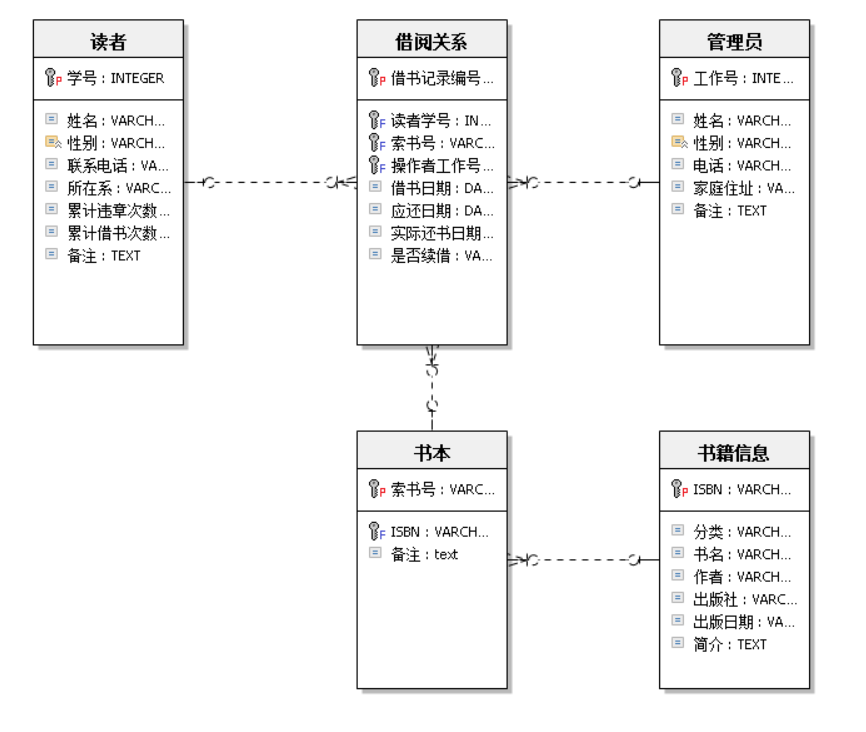
\includegraphics[scale=0.75]{db_imgs/logic1.PNG}
\end{figure}

\newpage


\subsection{数据库物理结构设计}

数据库物理结构由数据库逻辑结构自动转换生成。

\begin{figure}[!h]
\centering
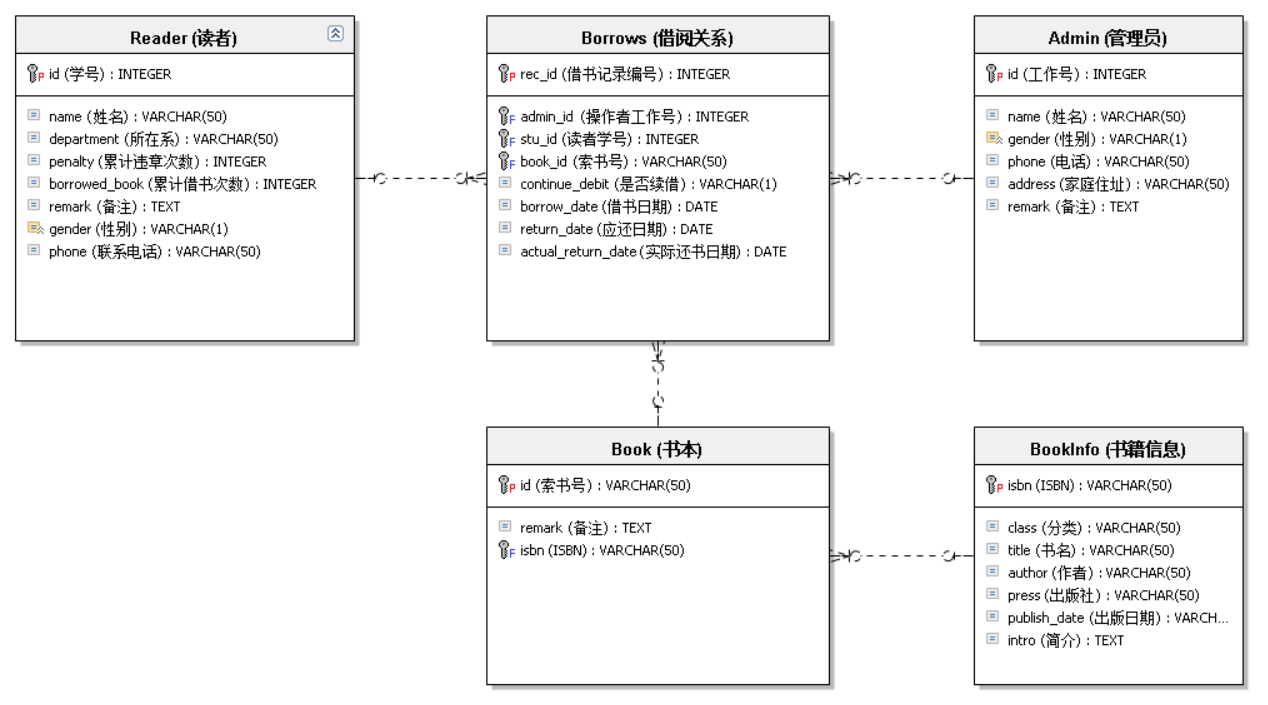
\includegraphics[scale=0.5]{db_imgs/logic2.PNG}
\end{figure}

\subsection{数据库模式 SQL 语句生成}

在 Datablau 中生成 Mysql 脚本:

\begin{figure}[!h]
\centering
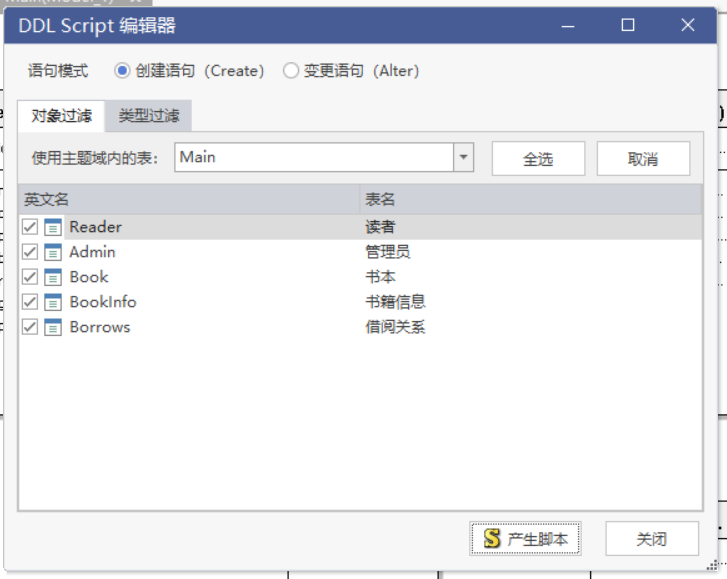
\includegraphics[scale=0.5]{db_imgs/script.PNG}
\end{figure}

生成一个 sql 文件:

\begin{lstlisting}[language=sql]
/*=================================================*/
/* Table: BookInfo
/* Definition: 
/* Author: gzez2012@163.com
/*=================================================*/
CREATE TABLE IF NOT EXISTS `BookInfo` (
	`isbn`	VARCHAR(50)	NOT NULL	COMMENT 'ISBN',
	`class`	VARCHAR(50)	COMMENT '分类',
	`title`	VARCHAR(50)	COMMENT '书名',
	`author`	VARCHAR(50)	COMMENT '作者',
	`press`	VARCHAR(50)	COMMENT '出版社',
	`publish_date`	VARCHAR(50)	COMMENT '出版日期',
	`intro`	TEXT	COMMENT '简介',
	PRIMARY KEY (`isbn`)
)
ENGINE=InnoDB
DEFAULT CHARACTER SET = utf8
COLLATE=utf8_bin
COMMENT='书籍信息';
/*=================================================*/
/* Table: Reader
/* Definition: 
/* Author: gzez2012@163.com
/*=================================================*/
CREATE TABLE IF NOT EXISTS `Reader` (
	`id`	INTEGER	NOT NULL	COMMENT '学号',
	`name`	VARCHAR(50)	NOT NULL	COMMENT '姓名',
	`department`	VARCHAR(50)	COMMENT '所在系',
	`penalty`	INTEGER	NOT NULL	DEFAULT '0'	COMMENT '累计违章次数',
	`borrowed_book`	INTEGER	NOT NULL	DEFAULT '0'	COMMENT '累计借书次数',
	`gender`	VARCHAR(1)	COMMENT '性别||CU0097',
	`phone`	VARCHAR(50)	COMMENT '联系电话',
	`remark`	TEXT	COMMENT '备注',
	PRIMARY KEY (`id`)
)
ENGINE=InnoDB
DEFAULT CHARACTER SET = utf8
COLLATE=utf8_bin
COMMENT='读者';
/*=================================================*/
/* Table: Admin
/* Definition: 
/* Author: gzez2012@163.com
/*=================================================*/
CREATE TABLE IF NOT EXISTS `Admin` (
	`id`	INTEGER	NOT NULL	COMMENT '工作号',
	`name`	VARCHAR(50)	NOT NULL	COMMENT '姓名',
	`gender`	VARCHAR(1)	COMMENT '性别||CU0097',
	`phone`	VARCHAR(50)	COMMENT '电话',
	`address`	VARCHAR(50)	COMMENT '家庭住址',
	`remark`	TEXT	COMMENT '备注',
	PRIMARY KEY (`id`)
)
ENGINE=InnoDB
DEFAULT CHARACTER SET = utf8
COLLATE=utf8_bin
COMMENT='管理员';
/*=================================================*/
/* Table: Book
/* Definition: 
/* Author: gzez2012@163.com
/*=================================================*/
CREATE TABLE IF NOT EXISTS `Book` (
	`id`	VARCHAR(50)	NOT NULL	COMMENT '索书号',
	`isbn`	VARCHAR(50)	NOT NULL	COMMENT 'ISBN',
	`remark`	TEXT	COMMENT '备注',
	PRIMARY KEY (`id`),
	CONSTRAINT `fk_Book_4` FOREIGN KEY (`isbn`) REFERENCES `BookInfo`(`isbn`)
)
ENGINE=InnoDB
DEFAULT CHARACTER SET = utf8
COLLATE=utf8_bin
COMMENT='书本';
/*=================================================*/
/* Table: Borrows
/* Definition: 
/* Author: gzez2012@163.com
/*=================================================*/
CREATE TABLE IF NOT EXISTS `Borrows` (
	`rec_id`	INTEGER	NOT NULL	COMMENT '借书记录编号',
	`stu_id`	INTEGER	NOT NULL	COMMENT '读者学号',
	`book_id`	VARCHAR(50)	NOT NULL	COMMENT '索书号',
	`admin_id`	INTEGER	NOT NULL	COMMENT '操作者工作号',
	`continue_debit`	VARCHAR(1)	NOT NULL	DEFAULT 'N'	COMMENT '是否续借',
	`borrow_date`	DATE	NOT NULL	COMMENT '借书日期',
	`return_date`	DATE	NOT NULL	COMMENT '应还日期',
	`actual_return_date`	DATE	COMMENT '实际还书日期',
	PRIMARY KEY (`rec_id`),
	CONSTRAINT `fk_Borrows_2` FOREIGN KEY (`book_id`) REFERENCES `Book`(`book_id`),
	CONSTRAINT `fk_Borrows_3` FOREIGN KEY (`stu_id`) REFERENCES `Reader`(`stu_id`),
	CONSTRAINT `fk_Borrows_4` FOREIGN KEY (`admin_id`) REFERENCES `Admin`(`admin_id`)
)
ENGINE=InnoDB
DEFAULT CHARACTER SET = utf8
COLLATE=utf8_bin
COMMENT='借阅关系';
\end{lstlisting}

\subsection{实验总结}

这个实验让我开始接触数据库设计软件,从用户需求来建模。常规思路是先列出数据实体,然后找出数据实体之间的关系,画出 E-R 图。为了减少数据冗余,我们还要使用BC范式 / 第三范式对数据表进行再拆分。然后再使用数据库设计软件进行数据库逻辑结构设计,再自动转换为数据库物理结构,最后生成 SQL 语句。

\end{document}
